%%%%%%%%%%%%%%%%%%%%%%%%%%%%%%%%%%%%%%%%%%%%%%%%%%%%%%%%%%%%%%%%%%%%%%%%%%%%%%%%%%%%%%%%%%%%%%%%%%%%%%%
%%													%%
%% 	BAKALÁŘSKÁ PRÁCE -  Zásuvný modul QGIS pro terénní radiační průzkum			%%
%% 				 Tereza Kulovaná							%%
%%													%%
%% pro formátování využita šablona: http://geo3.fsv.cvut.cz/kurzy/mod/resource/view.php?id=775 	%%
%%													%%
%%%%%%%%%%%%%%%%%%%%%%%%%%%%%%%%%%%%%%%%%%%%%%%%%%%%%%%%%%%%%%%%%%%%%%%%%%%%%%%%%%%%%%%%%%%%%%%%%%%%%%% 

\documentclass[%
  12pt,         			% Velikost základního písma je 12 bodů
  a4paper,      			% Formát papíru je A4
  oneside,       			% Oboustranný tisk
  pdftex,				    % překlad bude proveden programem 'pdftex' do PDF
%%%  draft
]{report}       			% Dokument třídy 'zpráva'
%

\newcommand{\Fbox}[1]{\fbox{\strut#1}}

\usepackage[czech, english]{babel}	% použití češtiny, angličtiny
\usepackage[utf8]{inputenc}		% Kódování zdrojových souborů je UTF8

\usepackage[square,sort,comma,numbers]{natbib}

\usepackage{caption}
\usepackage{subcaption}
\captionsetup{font=small}
\usepackage{enumitem} 
\setlist{leftmargin=*} % bez odsazení

\makeatletter
\setlength{\@fptop}{0pt}
\setlength{\@fpbot}{0pt plus 1fil}
\makeatletter

\usepackage[dvips]{graphicx}   
\usepackage{color}
\usepackage{transparent}
\usepackage{wrapfig}
\usepackage{float} 

\usepackage{cmap}           
\usepackage[T1]{fontenc}    

\usepackage{textcomp}
\usepackage[compact]{titlesec}
\usepackage{amsmath}
\addtolength{\jot}{1em} 

\usepackage{chngcntr}
\counterwithout{footnote}{chapter}

\usepackage{acronym}

\usepackage[
    unicode,                
    breaklinks=true,        
    hypertexnames=false,
    colorlinks=true, % true for print version
    citecolor=black,
    filecolor=black,
    linkcolor=black,
    urlcolor=black
]{hyperref}         

\usepackage{url}
\usepackage{fancyhdr}
%\usepackage{algorithmic}
\usepackage{algorithm}
\usepackage{algcompatible}
\renewcommand{\ALG@name}{Pseudokód}% Update algorithm name
\def\ALG@name{Pseudokód}

\usepackage[
  cvutstyle,          
  bachelor           
]{thesiscvut}


\newif\ifweb
\ifx\ifHtml\undefined % Mimo HTML.
    \webfalse
\else % V HTML.
    \webtrue
\fi 

\renewcommand{\figurename}{Obrázek}
\def\figurename{Obrázek}

%%%%%%%%%%%%%%%%%%%%%%%%%%%%%%%%%%%%%%%%%%%%%%%%%%%%%%%%%%%%%%%%%
%%%%%%%%%%% Definice informací o dokumentu  %%%%%%%%%%%%%%%%%%%%%
%%%%%%%%%%%%%%%%%%%%%%%%%%%%%%%%%%%%%%%%%%%%%%%%%%%%%%%%%%%%%%%%%

%% Název práce
\nazev{Zásuvný modul QGIS pro~terénní radiační průzkum}
{Radiation Reconnaissance Results to MGRS-described Polygon QGIS Plugin}

%% Jméno a příjmení autora
\autor{Tereza}{Kulovaná}

%% Jméno a příjmení vedoucího práce včetně titulů
\garant{Ing.~Martin~Landa,~Ph.D.}

%% Označení programu studia
\programstudia{Geodézie a~kartografie}{}

%% Označení oboru studia
\oborstudia{Geodézie, kartografie a~geoinformatika}{}

%% Označení ústavu
\ustav{Katedra geomatiky}{}

%% Rok obhajoby
\rok{2017}

%Mesic obhajoby
\mesic{červen}

%% Místo obhajoby
\misto{Praha}

%% Abstrakt
\abstrakt {Tato bakalářská práce je zaměřena na~automatizaci
  zpracování naměřených dat při~terénním radiačním průzkumu. Požadavek
  na~tento nástroj vzešel ze~strany Armády České republiky, jelikož
  v~době zadání práce celý postup prováděl operátor ručně. Nástroj je
  s~využitím externí knihovny implementován do~prostředí open source
  systému QGIS.}  {Abstract english}

%% Klíčová slova
\klicovaslova
{QGIS, zásuvný~modul, Python, GDAL, radiace}
{QGIS, plugin, Python, GDAL, radiation}

%%%%%%%%%%%%%%%%%%%%%%%%%%%%%%%%%%%%%%%%%%%%%%%%%%%%%%%%%%%%%%%%%%%%%%%%

%%%%%%%%%%%%%%%%%%%%%%%%%%%%%%%%%%%%%%%%%%%%%%%%%%%%%%%%%%%%%%%%%%%%%%%%
%% Nastavení polí ve Vlastnostech dokumentu PDF
%%%%%%%%%%%%%%%%%%%%%%%%%%%%%%%%%%%%%%%%%%%%%%%%%%%%%%%%%%%%%%%%%%%%%%%%
\nastavenipdf
%%%%%%%%%%%%%%%%%%%%%%%%%%%%%%%%%%%%%%%%%%%%%%%%%%%%%%%%%%%%%%%%%%%%%%%

%%% Začátek dokumentu
\begin{document}

\catcode`\-=12  % pro vypnuti aktivniho znaku '-' pouzivaneho napr. v \cline 

% aktivace záhlaví
\zahlavi

% předefinování vzhledu záhlaví
\renewcommand{\chaptermark}[1]{%
	\markboth{\MakeUppercase
	{%
	\thechapter.%
	\ #1}}{}}

% Vysázení přebalu práce
%\vytvorobalku

% Vysázení titulní stránky práce
\vytvortitulku

% Vysázení listu zadani
\stranka{}%
	{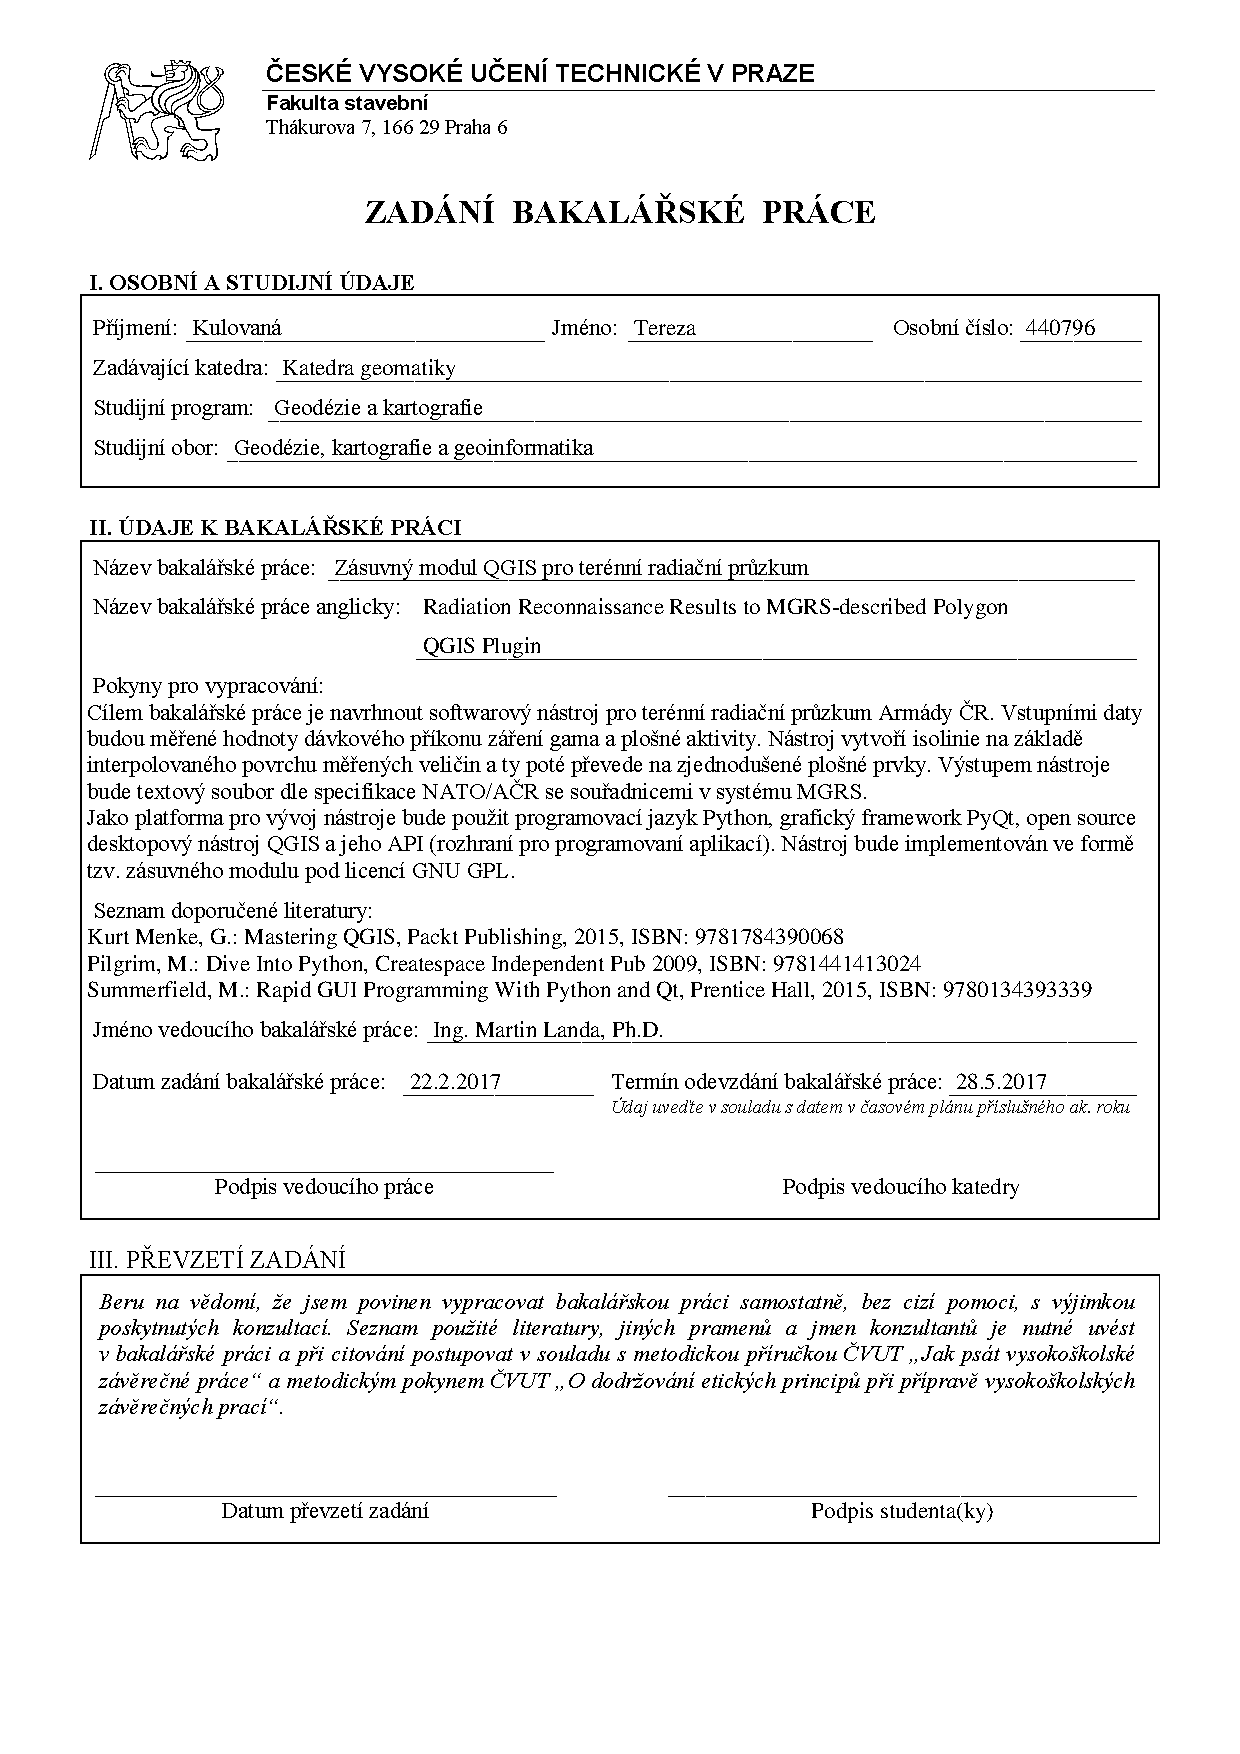
\includegraphics[scale=0.7]{./pictures/zadani.pdf}}%\sffamily\Huge\centering\ }%ZDE VLOŽIT LIST ZADÁNÍ}%
	%{\sffamily\centering Z~důvodu správného číslování stránek}

% Vysázení stránky s abstraktem
\vytvorabstrakt

% Vysázení prohlaseni o samostatnosti
\vytvorprohlaseni

% Vysázení poděkování
\stranka{%nahore
       }{%uprostred
       }{%dole
       \sffamily
	\begin{flushleft}
		\large
		\MakeUppercase{Poděkování}
	\end{flushleft}
	\vspace{1em}
		%\noindent
	\par\hspace{2ex}
	{Ráda bych poděkovala ... }
}

% Vysázení obsahu
\obsah

% Vysázení seznamu obrázků
\seznamobrazku

% Vysázení seznamu tabulek
\seznamtabulek

% jednotlivé kapitoly
\chapter{Úvod}
\label{1-uvod}

Hrozba jaderného výbuchu či jaderné havárie se v
posledních sto letech stala více než reálnou. Proto ve světě vznikla
potřeba být na takovéto situace co nejlépe připraven. V první řadě
existuje samozřejmě snaha jim předcházet, avšak pokud již některý 
ze~zmíněných stavů nastane, je důležité na něj reagovat rychle a
efektivně.  Důsledkem jsou snahy o zjednodušení získávání informací,
automatizaci jejich zpracování a standardizaci formátu, v němž jsou
předávány navazujícím složkám soustavy. Jedním ze způsobů, jak do
%%% ML: slovo obrovsky by bylo dobre nahradit vhodnejsim ekvivalentem
tohoto velkého a provázaného systému přispět, je i softwarový
nástroj, jehož vytvoření v rámci této bakalářské práce zadala Armáda
České republiky, přesněji 314. centrum výstrahy proti zbraním
hromadného ničení v Hostvici.

314. centrum výstrahy \zk{ZHN} je podřízeno 31. pluku radiační,
chemické a bio\-logické ochrany v Liberci. V Armádě ČR plní funkci
související se sledováním a~vyhodnocováním informací v oblasti
radiační, chemické a biologické ochrany.

V období míru je úkolem 314. centra mimo jiné spravovat armádní
radiační monitorovací síť Armády České republiky, provádět letecký
radiační průzkum, shromažďovat informace o zbraních hromadného ničení,
jaderných energetických zařízeních a navrhovat ochranná opatření proti
\zk{ZHN} či ochranu proti následkům radiačních havárií. "Při vyhlášení
stavu ohrožení státu/válečného stavu přebírá centrum od Ministerstva
vnitra úkoly ústředního koordinačního orgánu v oblasti moni\-torování a
výstrahy". \cite{ZHN}

V současnosti AČR zpracovává hodnoty naměřené v rámci radiačního
průzkumu ručně, za výpočty a zakreslení výsledků do mapy je zodpovědná
analytická skupina. Tento proces je poměrně náročný na znalosti a
zkušenosti operátora, ani čas strávený vyhodnocením není
zanedbatelný. Výhodný by proto byl softwarový nástroj, který by část
procesu zautomatizoval. Konkrétně se jedná o vytvoření
předdefinovaných izolinií ze vstupního interpolovaného gridu, jejich
převod na zjednodušené polygony a vygenerování textového reportu ve
%%% ML: souradnicovy nebo hlasny?
%%% TK: spravne ma byt hlasny
formátu dle specifikace \zk{NATO}/\zk{AČR} v hlásném systému
\zk{MGRS}. Na operátorovi pak zůstane následné vložení zprávy do
softwaru určeného k varování a uvědomování ostatních jednotek.

S ohledem na skutečnost, že \zk{AČR} zpracovává data v open source
geografickém informačním systému QGIS, bylo rozhodnuto, že nástroj
bude vyvíjen jako nový zásuvný modul pro toto prostředí. Modul bude
psán v programovacím jazyku Python, pro grafické rozhraní bude použit
framework Qt, bude využívat QGIS \zk{API}. Pro své specializované
funkce je uvažováno i využití GRASS GIS \zk{API} a knihovna \zk{GDAL}.

V teoretické části práce bude čtenář seznámen se způsoby monitorování
radiační situace v České republice, dotkne se tématu standardizovaných
%%% ML: hlásný ?
zpráv předávaných v rámci armády a představí hlásný systém \zk{MGRS}.

\textbf{Rešerše:} Z českých prací se zadanému tématu z hlediska teorie
nejvíce blíží diplomová práce Bc. Romany Loškové \textit{Hodnocení
přístrojů používaných v AČR v~případě mimořádné radiační
události}\footnote{\url{http://theses.cz/id/o3vhp8/Diplomov_prce_Lokov.pdf}}. Zabývá
se monitorováním radiační situace a~přístroji používanými v rámci
\zk{AČR}. Naopak z hlediska praktické části je nejpodobnější
bakalářská práce Ondřeje Peška \textit{Posun letecky měřených bodů po
  trajektorii v prostředí
  %%% ML: nahradil jsem neoficialnim odkazem, ktery je uchopitelnejsi 
QGIS}\footnote{\url{https://github.com/ctu-osgeorel-proj/bp-pesek-2016/raw/master/text/ondrej-pesek-bp-2016.pdf}},
která byla vedena v roce 2016 na katedře geomatiky FSv ČVUT. Jejím
cílem je také vytvoření zásuvného modulu pro QGIS.
\chapter{Teoretický základ}
\label{2-teorie}

V této kapitole jsou objasněny způsoby monitorování radiační situace, popsán sběr dat a představen výstupní report.

\section{Ionizující záření}

Ionizující záření je tok buď hmotných částic, nebo fotonů elektromagnetického záření, které mají schopnost ionizovat atomy prostředí či excitovat jejich jádra. Příčinou vzniku může být radioaktivní rozpad, kosmické záření nebo jej lze vytvořit uměle. Je průvodním jevem jaderných procesů, během nichž se jádro či obal atomu dostávají do energeticky nestabilního excitovaného stavu. Pro návrat do stabilního stavu musí vyzářit energii ve formě částic či fotonů elektromagnetického záření. Podle způsobu interakce s prostředím se ionizující záření dělí na dva druhy:

\begin{itemize}
	\item \textbf{Přímo ionizující záření} mohou způsobovat jen nabité částice, které mají dostatečnou kinetickou energii k vyvolání ionizace. Mezi nabité částice patří např. elektrony, částice $\alpha$, $\beta$.
	
	\item \textbf{Nepřímo ionizující záření} je tvořeno nenabitými částicemi (neutrony, fotony), které prostředí přímo sami neionizují, ale při vzájemném působení s prostředím předávají svou kinetickou energii sekundárním, nabitým částicím, jež následně přímými účinky na atomy látku ionizují.
\end{itemize}

% http://astronuklfyzika.cz/JadRadFyzika6.htm
% http://fbmi.sirdik.org/1-kapitola/13/131.html

\subsection{Fyzikální veličiny a jednotky}

\begin{itemize}
	\item \textbf{Plošná aktivita}
	
	Množství radioaktivní látky je charakterizováno aktivitou. Jedná se o počet radioaktivních přeměn vztažených na jednotku času. Aktivita má za jednotku becquerel {[}Bq{]}. U plošných zdrojů záření se používá plošná aktivita neboli podíl aktivity a celkové plochy látky {[}Bq/m$^2${]}.
	
	\item \textbf{Dávkový příkon}
	
	Působení ionizujícího záření popisuje veličina dávka (či také absorbovaná dávka), která je určena jako poměr střední energie předané ionizujícím zářením látce o dané hmotnosti. Základní jednotkou je gray {[}Gy{]}, který odpovídá energii 1 joule absorbované v kilogramu látky. Dávkový příkon je přírůstek dávky v časovém intervalu {[}Gy/s{]}. V praxi se používají nižší jednotky {[}µGy/h{]} nebo {[}cGy/h{]}.

	\item \textbf{Příkon dávkového ekvivalentu}
	
	Na rozdíl od předchozích veličin patří dávkový ekvivalent mezi tzv. radiobiologické veličiny, tj. zohledňující účinky působení různých druhů záření na živou hmotu. Dávkový ekvivalent je součin dávky v uvažovaném bodě tkáně a jakostního činitele, jenž vyjadřuje rozdílnou biologickou účinnost různých druhů záření. Příkon fotonového dávkového ekvivalentu (\zk{PFDE}) je přírůstek dávkového ekvivalentu způsobeného fotony v časovém intervalu {[}Sv/s{]}. Prostorový dávkový ekvivalent odpovídá dávkovému ekvivalentu, který by uspořádané a rozšířené pole ionizujícího záření způsobilo v hloubce d = 10 mm v ICRU kouli\footnote{Koule z materiálu adekvátně odpovídajícího tkáni lidského těla o průměru 30 cm} na rádius vektoru opačného směru, než je orientované pole. Příkon prostorového dávkového ekvivalentu (\zk{PPDE}) je přírůstek prostorového dávkového ekvivalentu v časovém intervalu {[}Sv/s{]}.
% http://www.radioaktivita.cz/jednotky.html
% https://www.sujb.cz/aplikace/monras/?lng=cs_CZ#z3
%http://fbmi.sirdik.org/

		\begin{table}[h!]
			\centering
			\caption{Fyzikální veličiny}
			\label{tab:tab_veliciny}
			\begin{tabular}{|c|c|c|}
				\hline
				\textbf{Veličina}           			& \textbf{Jednotka}  & \textbf{Značka}  \\ \hline
				Aktivita								& becquerel			 & {[}Bq{]}			\\ \hline
				Plošná aktivita							& becquerel/m$^2$	 & {[}Bq/m$^2${]}	\\ \hline
				Dávka                      	 			& gray               & {[}Gy{]}         \\ \hline
				Dávkový příkon              			& gray/sekunda		 & {[}Gy/s{]}       \\ \hline
				Dávkový ekvivalent          			& sievert            & {[}Sv{]}         \\ \hline
				Příkon fotonového dávkového ekvivalentu & sievert/sekunda	 & {[}Sv/s{]}       \\ \hline
				Příkon prostorového dávkového ekvivalentu & sievert/sekunda	 & {[}Sv/s{]}       \\ \hline
			\end{tabular}
		\end{table}
\end{itemize}

\section{Monitorování radiační situace}
% (50) https://www.sujb.cz/aplikace/monras/?lng=cs_CZ#z0

Pod monitorováním radiační situace je myšleno pravidelné sledování úrovně ionizujícího záření v okolním prostředí, měření obsahu umělých radionuklidů ve složkách životního prostředí a potravních řetězců, ale také sledování radioaktivity v těle člověka. (50)

Systematické plošné monitorování radiační situace má na území České republiky počátky v dubnu 1986, kdy došlo k havárii v \zk{JE} Černobyl. Je zajišťováno pomocí celostátní Radiační monitorovací sítě (\zk{RMS}) spravované Státním ústavem pro jadernou bezpečnost (\zk{SÚJB}).

\zk{RMS} běžně operuje v tzv. normálním režimu, v případě mimořádné radiační situace přechází do tzv. havarijního režimu. Během normálního režimu pracují stálé složky \zk{RMS}, jež v první řadě zajišťují provoz fixních měřících míst a analýzu dat z nich získaných. Mezi stálé složky \zk{RMS} patří v první řadě \zk{SÚJB}, Státní ústav radiační ochrany (\zk{SÚRO}) a Český hydrometeorologický úřad (\zk{ČHMÚ}). Při přechodu do havarijního režimu dochází rovněž k aktivaci pohotovostních složek. Po zvážení je zahájen radiační průzkum, který sestává z dalšího monitorování na měřících bodech, pojezdového měření a v případě potřeby i měření leteckého. (2) Všechny získané informace jsou potřebné pro rozhodování o opatřeních vedoucích ke snížení nebo odvrácení ozáření.

% (1) http://www.mocr.army.cz/informacni-servis/zpravodajstvi/chemici-se-specialisty-statniho-ustavu-radiacni-ochrany-spolecne-monitorovali-radiaci-z-vrtulniku-118918/

% (2) https://www.suro.cz/cz/rms	

\subsection{Sběr dat}	

Mezi hlavní způsoby monitorování radiační situace patří:

\begin{itemize}
	\item \textbf{napevno umístěné detektory (měřící body)}
	
\begin{figure}[H]
    \centering
      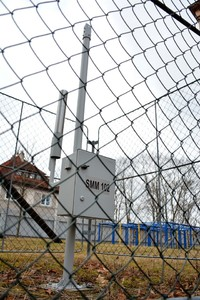
\includegraphics[width=150pt]{./pictures/03_merici-sonda-v-libereckych-kasarnach_2.jpg}
      \caption[Měřící sonda libereckých chemiků]{Měřící sonda libereckých chemiků
      (autor: \href{http://www.acr.army.cz/informacni-servis/zpravodajstvi/armadni-radiacni-monitorovaci-site-nacvicoval-zasah-pri-radiaci-131355/}{kapitán Ing. Jakub Šimíček})}
      \label{fig:sonda}
\end{figure}
	
	Jedním ze způsobů hodnocení radiační situace je zjištění odchylek od dlouhodobého průměru \zk{PFDE}, resp. \zk{PPDE}. Dlouhodobě měřené hodnoty \zk{PFDE} na území České republiky se pohybují mezi 0,1 až 0,2 {[}µSv/h{]}\footnote{Zdroj: https://www.sujb.cz/aplikace/monras/}. Tato měření jsou nepřetržitě prováděna na pevně umístěných detektorech.
	
	Základním systémem, umožňujícím průběžné sledování radiační situace na území ČR, je Síť včasného zjištění (\zk{SVZ}) spravovaná Regionálními centry (RC) \zk{SÚJB}, \zk{SÚRO}, \zk{ČHMÚ} a Armádou ČR. SVZ je v okolí a uvnitř areálu jaderných elektráren Dukovany a Temelín doplněna teledozimetrickými systémy (\zk{TDS}), jejichž činnost je zajišťována ČEZ, a.s. Detekční jednotky \zk{SVZ} i \zk{TDS} obsahují dva detektory s různým rozsahem měření veličiny \zk{PFDE}. Dalším způsobem zjištění odchylek od průměru jsou integrální měření fotonových, resp. prostorových dávkových ekvivalentů zjišťovaná v měřících místech s integrálními dozimetry, které tvoří teritoriální síť a lokální síť v okolí \zk{JE}.
	
		
	\item \textbf{pozemní monitorování}
	
\begin{figure}[H]
    \centering
      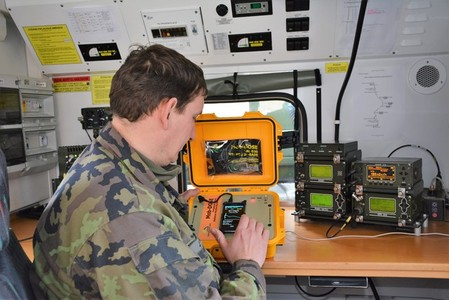
\includegraphics[width=250pt]{./pictures/02_mereni-radiace-v-terenu-z-vozidla_2.jpg}
      \caption[Liberecký chemik měří radiaci v terénu ve speciálním vozidle]{Liberecký chemik měří radiaci v terénu ve speciálním vozidle
      (autor: \href{http://www.acr.army.cz/informacni-servis/zpravodajstvi/armadni-radiacni-monitorovaci-site-nacvicoval-zasah-pri-radiaci-131355/}{kapitán Ing. Jakub Šimíček})}
      \label{fig:pozemni}
\end{figure}
	
	Sběr dat při pojezdovém měření je prováděn z vozidla jedoucího rychlostí 40 km/h po určené trase. Spolu s měřenou hodnotou se zaznamenává čas a poloha měření.
	
	Při naměření předem stanoveného dávkového příkonu osádka vozu již dále nepokračuje ve směru rostoucích hodnot do epicentra výbuchu. "Takováto úroveň se pouze vytyčí a souřadnice jejího naměření se zahlásí radiostanicí na sběrné stanoviště (veliteli jednotky radiačního průzkumu, popřípadě na analytickou skupinu)," popisuje nadporučík Jiří Komárek, starší důstojník Skupiny monitorování a leteckého průzkumu 314. centra výstrahy \zk{ZHN}. Následně se osádka vrací zpět po stejné trase. 
	
	Právě závislost pozemního průzkumu na trasách přesunu, tj. cestách, a vystavení osádky vyšším hodnotám ionizujícího záření je jeho největší nevýhodou. Proto se provádí jako doplněk k měření leteckému. Hlavním zdrojem informací se stává ve chvíli, kdy povětrnostní podmínky nedovolí realizovat letecké monitorování.
	
	Pozemní monitorování zajišťují \zk{SÚJB}, \zk{SÚRO}, Hasičský záchranný sbor ČR, Generální ředitelství cel, Armáda ČR, Policie ČR a ČEZ, a.s. 
	
	\item \textbf{letecké monitorování}
	
	Letecké monitorování je prováděno z vrtulníku letícího ve výšce asi 100 m nad terénem po předem určených trasách. Naměřené údaje jsou přepočítány na úroveň radiace ve výšce 1 m nad terénem. Oproti pojezdovému měření si letecký průzkum může dovolit prozkoumat kontaminovaný prostor více do hloubky. Úkolem specialistů na palubě však je sledování měřených dávkových příkonů, aby eventuálně mohli buď upravit parametry průzkumu (rychlost, výška letu), nebo změnit trasu letu. Cílem je rychlé, orientační zmapování velké oblasti bez ohledu na charakter terénu. 
	
	"V případě jaderného výbuchu by mohl být letecký průzkum potenciálně využit ke zmapování radioaktivní stopy, kterou takový výbuch po vypadání částic zanechá. Důležité jsou tady samozřejmě vhodně zvolené podmínky průzkumu," doplňuje dále nadporučík Komárek. 
	
	Omezujícími podmínkami leteckého průzkumu je povětrnostní situace a doba, po kterou je třeba vyčkat, než vypadají radioaktivní částice na zemský povrch. Během čekání lze předběžně určit orientační dávkové příkony v epicentru vztažené na odhad mohutnosti výbuchu, na jejichž základě se rozhodne o provedení průzkumu ve vhodném časovém horizontu (po "vymření" krátkodobých radionuklidů, kdy radiace v epicentru poklesne). Následně lze provést průzkum v souladu s principem \zk{ALARA}, tedy že dávka ionizujícího záření, které je osoba vystavena, má být tak nízká, jaké lze rozumně dosáhnout.
	
	Letecké monitorování v ČR provádí \zk{SÚRO} a Armáda ČR. 

\end{itemize}
	
	Nově získané hodnoty radiačního monitorování jsou při vkládání do programu \zk{MonRaS} porovnávány s informačními úrovněmi. Informační úrovně existují dvě: 1. a 2. IU. Při jejich překročení jsou zjišťovány důvody jejich překročení a případně provedeny kroky nutné k odstranění příčiny.
	
\subsection{Armádní radiační monitorovací síť}	
	
% zdroj: JK
% http://www.vvubrno.cz/userstorage/files/pdf/prospekty/svz-arms-sit-vcasneho-zjisteni.pdf
% http://www.acr.army.cz/informacni-servis/zpravodajstvi/armadni-radiacni-monitorovaci-site-nacvicoval-zasah-pri-radiaci-131355/
	
	U Armády České republiky se monitorováním radiační situace zabývají dvě jednotky. 
	 
	 314. centrum výstrahy proti zbraním hromadného ničení (\zk{ZHN}) v Hostivici-Břve je zodpovědné především za letecký radiační průzkum a monitorování radiační situace pomocí Sítě včasného zjištění patřící do Armádní radiační monitorovací sítě (\zk{SVZ ARMS}). Jedná se o soustavu 16 stacionárních sond (původně jich bylo 17, ale sonda v Rakovníku byla zrušena a dosud nebyla nahrazena). \zk{AČR} svými daty ze \zk{SVZ ARMS} přispívá do celostátní \zk{RMS}, kterou spravuje \zk{SÚJB}.
	 
	 K provedení leteckého radiačního průzkumu AČR využívá vrtulník Mi-17???. V současné době AČR disponuje gama spektrometrickým systémem IRIS (Integrated Radiation Information System), přístrojem MobDOSE a palubním detektorem DP-3a. IRIS umí měřit nejen dávkový příkon a dávku, ale především energetické spektrum detekovaného záření gama, tj. lze jej využít ke gama spektrometrii.
	
	 Za pozemní průzkum jsou zodpovědné především jednotky 31. pluku radiační, chemické a biologické ochrany v Liberci. Sběr dat při pojezdovém měření je prováděn z vozidla Land Rover LR-110, lehkého obrněného kolového transportéru BRDM-2 nebo džípu UAZ-469 (postupně vyřazován). Přístroje používané k měření dávkového příkonu jsou DP-98, AS-67 nebo DP-3b a jsou pevně spojené s vozidlem. 
	 
	 
\section{Textový report}
% JK
% https://systematic.com/defence/products/a/military-messaging/app-11-and-adatp-3/	

Týká se nová verze APP-11 mého výstupu???

APP-11 je katalog, který specifikuje formát textových zpráv (\zk{MTF}) používaných v \zk{NATO} ke komunikaci se spřátelenými silami. Poslední verze katalogu APP-11 obsahuje více než 400 zpráv pokrývajících každý aspekt operací NATO, při němž se vyskytuje potřeba předávání informací pomocí standardizovaných zpráv. Zprávy jsou sestaveny na základně pravidel uvedených v technické publikaci ADatP-3. 

\zk{MTF} zprávy se skládají ze dvou částí - hlavičky a těla. Hlavička zahrnuje data o původci, příjemci či klasifikaci. Tělo pak obsahuje předávanou informaci ve formátu specifikovaném v APP-11. 

\begin{figure}[H]
    \centering
      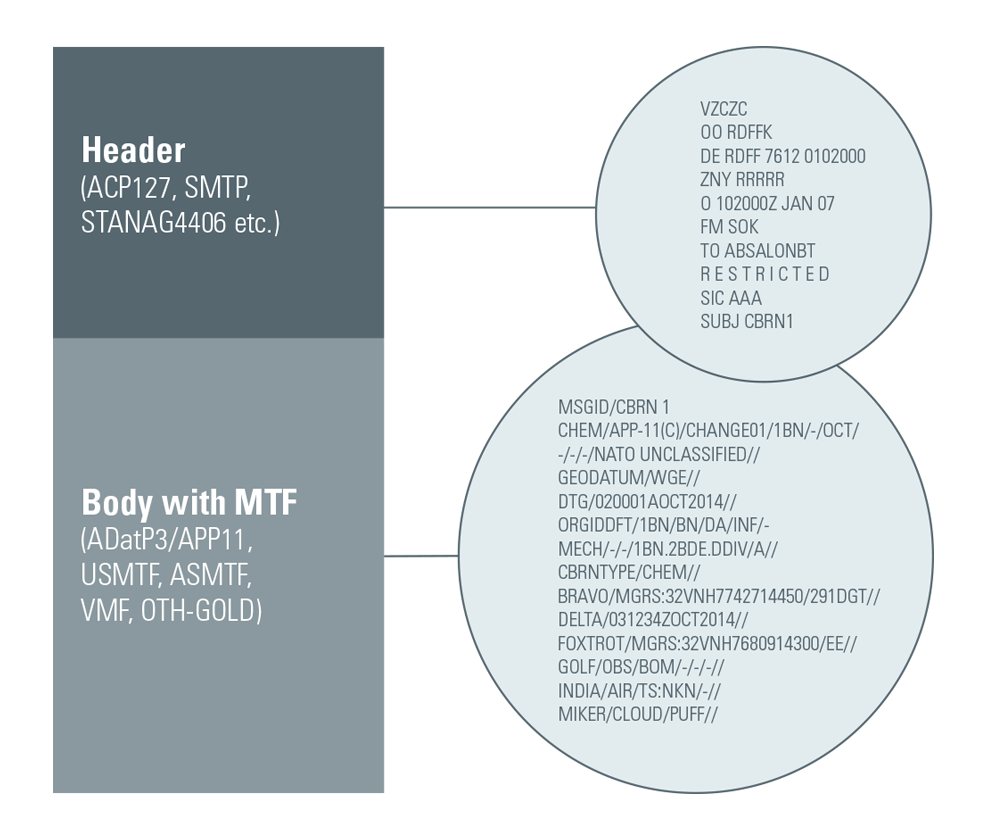
\includegraphics[width=300pt]{./pictures/Military-Messaging-white-borders-988px.png}
      \caption[Struktura zprávy MTF]{Struktura zprávy MTF
      (zdroj: \href{https://systematic.com/defence/products/a/military-messaging/app-11-and-adatp-3/}{SYSTEMATIC})}
      \label{fig:systematic}
  \end{figure}
  
Hlavní výhody \zk{MTF} zprávy:

\begin{itemize}
	\item \textbf{jasně strukturovaný obsah je pochopitelný a předchází nedorozuměním} 
	\item \textbf{je přenositelná mezi různými národy a systémy} 
	\item \textbf{při přenosu požaduje malou šířku vlnového pásma}
	\item \textbf{je vhodná pro strojové zpracování}
\end{itemize}

Výstupem ze zásuvného modulu je textový report ve formátu v souladu s katalogem APP-11. Jedná se o seznam souřadnic lomových bodů polygonů v systému \zk{MGRS}, který bude součástí \zk{MTF} zprávy. (viz Kapitola 4.4 Výstupní report)

\subsection{Military grid reference system}
Hlásný systém MGRS (\zk{MGRS}) je systém udávání polohy používaný Severoatlantickou aliancí (\zk{NATO}). Využívá Mercatorovo příčné válcové konformní zobrazení (\zk{UTM}), případně \zk{UPS}. 

Na rozdíl od jiných souřadnicových systémů, které vyjadřují polohu pomocí dvojice hodnot (šířka/délka, x/y), MGRS využívá jen jednu hodnotu a to alfanumerický řetězec znaků. Ten je tvořen třemi údaji:

\begin{itemize}
	\item \textbf{označení zóny}
	
	Jedna zóna je tvořena sférickým čtyřúhelníkem referenčního elipsoidu, jenž je vymezen zeměpisnými poledníky a rovnoběžkami. Sférické čtyřúhelníky vznikají rozdělením povrchu Země do 60 poledníkových zón o šířce 6°, které jsou následně děleny ve směru rovnoběžek na 19 vrstev po 8° a 1 vrstvu o výšce 12°.
	
	Poledníkové pásy jsou číslovány od 1 do 60 od obrazu poledníku 180° z. d. směrem na východ. Vrstvy jsou značeny velkými písmeny latinské abecedy C-X (s vynecháním písmen I a O vzhledem k jejich podobnosti s číslicemi) od obrazu rovnoběžky 80° j. š. na sever.
	
	Jedinečné označení zóny je složeno z čísla poledníkového pásu následovaného písmenem rovnoběžkového pásu (např. 33U).
	
	\item \textbf{označení čtverce 100 x 100 km}
	
	Jednotlivé zóny jsou rozděleny na čtverce o hraně 100 km sítí čar rovnoběžných s obrazem příslušného osového poledníku a rovníku. Jelikož se poledníkové pásy směrem k pólům zužují, zóny obsahují určitý počet úplných čtverců a na krajích neúplné čtverce o proměnlivé šířce. 
	
	Pro označení sloupců jsou použita písmena A-Z (s vynecháním I a O), značení začíná u obrazu poledníku 180° z. d. a pokračuje směrem na východ, po písmenu Z se celá řada opět opakuje. Vrstvám jsou přidělena písmena A-V (bez I a O). První vrstva lichých poledníkových pásů je značena písmenem A, u sudých pásů začíná písmenem F. Po písmenu V se abeceda opakuje. 
	
	Označení čtverce se skládá ze dvou písmen - označení sloupce a vrstvy (např. VR)
		
	\item \textbf{souřadnice bodu ve 100 km čtverci}
	
	V rámci čtverce je upřesněna poloha bodu za pomoci n+n číslic, kde první sada číslic určuje východní souřadnici od levého kraje čtverce a druhá sada severní souřadnici od okraje spodního. Podle přesnosti vyjádření polohy bodu n nabývá hodnot 1, 2, 3, 4 nebo 5. 
	
		\begin{itemize}
				\item 1+1 číslice pro souřadnici s přesností 10 km (\textit{54})
				\item 2+2 číslice pro souřadnici s přesností 1 km (\textit{5748})
				\item 3+3 číslice pro souřadnici s přesností 100 m (\textit{577484})
				\item 4+4 číslice pro souřadnici s přesností 10 m (\textit{57704840})
				\item 5+5 číslic pro souřadnici s přesností 1 m (\textit{5770048400})
		\end{itemize}	
		 
\end{itemize}

\begin{figure}[H]
    \centering
      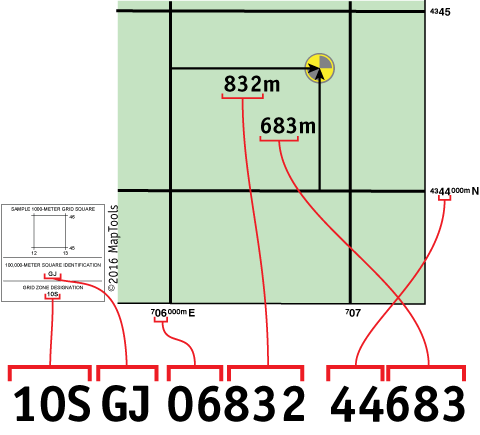
\includegraphics[width=250pt]{./pictures/MGRS_tvorba.png}
      \caption[Postup tvorby souřadnic MGRS]{Postup tvorby souřadnic MGRS
      (zdroj: \href{https://www.maptools.com/tutorials/mgrs/quick_guide}{MapTools})}
      \label{fig:maptools}
\end{figure}
  
Poloha Fakulty stavební ČVUT v Praze by tedy pomocí hlásného systému MGRS s přesností na metry byla vyjádřena řetězcem ...

Standardem NATO je rozlišení 10 m [wiki], Armáda ČR pro výstup zásuvného modulu požaduje přesnost na 1 m.

Východní a severní souřadnice v systému MGRS se vždy vztahují k levému dolnímu rohu čtverce. Při přechodu na nižší přesnost se souřadnice nezaokrouhlují, ale přebytečné číslice se odříznou, aby bylo zajištěno, že bod zůstane ve správném čtverci s nižší přesností.

% Souřadnice (například 33UVR577484, tj. 33U VR 577 484) se skládají z několika informací:



%zdroje: 
% https://boundlessgeo.com/2015/04/mgrs-coordinates-qgis/ - vlastně vůbec
% https://www.vugtk.cz/slovnik/5479_hlasny-system-mgrs - základní definice
% http://uhulag.mendelu.cz/files/pagesdata/cz/geodezie/geodezie1/souradnicove_systemy.pdf (str. 48)
% http://www.diverzanti.cz/cl_36a - nejvíc
% https://en.wikipedia.org/wiki/Military_Grid_Reference_System

\chapter{Použité technologie}
\label{3-technologie}

Třetí kapitola stručně představuje jednotlivé technologie použité při
tvorbě zásuvného modulu.

\section{QGIS}

\begin{figure}[H] \centering
      
\includegraphics[width=200pt]{./pictures/qgis-logo.png}
      \caption[QGIS logo]{QGIS logo (zdroj:
\href{https://www.qgis.org/en/_downloads/qgis-logo.png}{QGIS})}
      \label{fig:qgis}
  \end{figure}

QGIS (dříve známý pod názvem Quantum GIS) je multiplatformní volně
dostupný geografický informační systém (\zk{GIS}). Umožňuje uživateli
prohlížet, vytvářet, analyzovat a editovat jak vektorová, tak rastrová
geografická data.

Vývoj započal v roce 2002 Gary Sherman, dnes ho spravuje skupina
dobrovolníků a je vyvíjen pod hlavičkou Open Source Geospatial
Foundation (\zk{OSGeo}). Hlavní myšlenkou při vzniku bylo vytvoření
GIS softwaru dostupného zdarma každému vlastníkovi osobního počítače,
na rozdíl od drahých komerčních softwarů. Ty ho ve všech aspektech
sice většinou předčí, avšak pro běžného uživatele je QGIS zcela
dostačující.

QGIS je vyvíjen v jazyku C++, jeho grafické rozhraní využívá knihovnu
Qt. Je podporován na operačních systémech Microsoft Windows, Mac OS X,
Linux a Unix, od roku 2014 existuje experimentální verze pro
Android\footnote{\url{http://www.qgis.org/en/site/forusers/download.html}}. Základní
funkcionalitu pomáhají rozšířit zásuvné moduly psané v jazyce Python
nebo C++. Je propojen s dalšími open source GIS balíčky jako jsou
např. GRASS GIS, PostGIS nebo MapServer. QGIS je uvolněn pod licencí
GNU (\zk{GPL}) verze 2 a vyšší. \cite{qgis}

Komunita kolem QGIS aktivně podporuje své členy k přispívání a
zlepšování softwaru - hlášením chyb, překládáním programu do dalších
jazyků nebo snadným přístupem k tvorbě zásuvných modulů a jejich
implementaci.

% (1) http://www.qgis.org/en/site/forusers/download.html

\section{Python}

\begin{figure}[H] \centering
      
\includegraphics[width=150pt]{./pictures/python-logo-master-v3-TM.png}
      \caption[Python logo]{Python logo (zdroj:
\href{https://www.python.org/static/community_logos/python-logo-master-v3-TM.png}{Python.org})}
      \label{fig:python}
  \end{figure}
  
Python je vysokoúrovňový, interpretovaný programovací jazyk. Podporuje
procedurálně i objektově orientované programování, je výkonný, zároveň
má velmi jednoduchou a čistou syntax. V ostatních jazycích je
odsazování řádků doporučeno z hlediska přehlednosti, u Pythonu je
základním stavebním kamenem a je povinné.

Guido van Rossum, autor první verze Pythonu vydané v roce 1991, se
rozhodl vyřešit nedostatečnost jazyků, které byly používány v jeho
zaměstnání, a napsat jazyk splňující jeho potřeby. Při vývoji se
inspiroval především v jazycích ABC a~Modula-3. Jednou ze snah bylo
vytvoření jazyka otevřeného dalším rozšířením a~propojením s jinými
jazyky (např. C++). Dnes je Python vyvíjen jako open source projekt
pod záštitou neziskové organizace Python Software Foundation
(\zk{PSF}). Je distribuován pod licencí \zk{PSF}, která je
kompatibilní s \zk{GPL}. Je možné ho nainstalovat na běžné platformy
jako Windows, Unix nebo Mac OS, pro Linux je většinou součástí
základní instalace. Při vyvarování se systémově závislých funkcí je
přenositelný mezi~platformami bez jakýchkoli změn.

Python má široké využití, od jednoduchých programů po rozsáhlé
aplikace. Právě pro tyto možnosti, univerzálnost, přehlednost kódu a
%%% ML: sila? ta veta zni divne
výkonnost z něj udělaly programovací jazyk, který je mezi začátečníky ve
velké oblibě. Během krátké doby v~něm funkční skript zvládne napsat
každý.
  
% (3) https://docs.python.org/3/faq/general.html#general-python-faq
  
\section{GDAL}
%%% ML: pridat logo? (pro zachovani konzistence)

\begin{figure}[H] \centering
      
\includegraphics[width=100pt]{./pictures/gdal_logo.png}
      \caption[GDAL logo]{GDAL logo (zdroj:
\href{https://cs.wikipedia.org/wiki/Soubor:GDALLogoColor.svg}{Wikimedia Commons})}
      \label{fig:gdal}
  \end{figure}
  
Geospatial Data Abstraction Library (\zk{GDAL}) je knihovna určená pro
čtení a zápis rastrových a vektorových geodat. Od verze GDAL 2.0 došlo
k pevnějšímu propojení dvou původně oddělených knihoven - GDAL,
pracující s rastrovými daty, a OGR, zpracovávající data vektorová.

Do verze 1.3.2 byla vyvíjena Frankem Warmerdamem. Další údržba byla
převedena na GDAL/OGR Project Management Committee, která je součástí
\zk{OSGeo} Foundation.

GDAL/OGR je napsána v jazyce ANSI C a C++ a lze ji použít na
operačních systémech Linux, Solaris, Mac OS X a Microsoft
%%% ML: (4) ???
%%% TK: doplněna správná citace
Windows. Knihovna GDAL je vydávána pod licencí X/MIT. Pro práci se
souřadnicovými systémy a transformaci mezi nimi využívá knihovnu
PROJ.4. V květnu 2017 byla vydána zatím poslední verze GDAL 2.2.0. 
\cite{gdal}

Díky rozsáhlému množství funkcionalit je využívána v komerční i
nekomerční sféře a v oblasti GIS patří mezi hlavní free software
projekty.

% (4) http://www.gdal.org/ (hlavní strana + FAQ)

\newpage
\section{Qt Project}

\begin{figure}[H] \centering
      
\includegraphics[width=100pt]{./pictures/qt_logo_green_256x256px.png}
      \caption[Qt Project logo]{Qt Project logo (zdroj:
\href{http://brand.qt.io/downloads/}{qt.io})}
      \label{fig:qt}
  \end{figure}

Qt je framework\footnote{Multiplatformní aplikační rámec} knihoven a
nástrojů, jenž je široce využíván pro tvorbu multiplatformních
aplikací a grafických uživatelských rozhraní. Svou oblibu si vysloužil
právě funkčností na různých softwarových i hardwarových platformách,
kdy je třeba do kódu zavést jen pár změn nebo ho neupravovat
vůbec. Další výhodou je velmi dobře zpracovaná dokumentace.

Qt je založen na jazyku C++. Na vývoji Qt se v současnosti podílejí
dvě společnosti - The Qt Company a Qt Project, z nichž druhá jmenovaná
následuje politiku otevřených dat. Qt je tedy dostupný jak pod
komerční licencí, tak pod open source licencemi GNU \zk{GPL} 2.0, GNU
\zk{GPL} 3.0 a \zk{LGPL} 3.0. Poslední verzí vydanou před květnem 2017
byla verze Qt 5.8. \cite{qt}

% (5) https://www.qt.io/company/

\subsection{PyQt} Qt je sice psán v jazyce C++, ale existuje mnoho
rozhraní pro programování aplikací (\zk{API}) umožňujících propojení s
dalšími programovacími jazyky. Pro Python patří mezi nejoblíbenější
PyQt a PySide.

Správa a vývoj PyQt spadá pod firmu Riverbank Computing Limited. PyQt
je dostupný pod podobnou licencí jako Qt, tedy GNU \zk{GPL} 2.0, GNU
\zk{GPL} 3.0 a~komerční licencí. \cite{pyqt}

% (6) https://wiki.python.org/moin/PyQt


\chapter{Zásuvný modul}
\label{4-plugin}

Ve této kapitole jsou objasněny stěžejní kroky tvorby zásuvného modulu
\textit{Radiation reconnaissance results}, popsány vstupní a výstupní
datové soubory. Při tvorbě modulu byly využívány příručky \cite{diveintopython} 
\cite{cookbook} \cite{qgis} \cite{ucebnicepython}.
%%% ML: vetu dokoncit...

\section{Vstupní data}

Na vstupu zásuvného modulu je buď interpolovaná mapa dávkového
příkonu, nebo plošné aktivity.

\begin{itemize}
\item \textbf{Interpolovaná mapa plošné aktivity}

  Mapa obsahuje hodnoty plošné aktivity v jednotkách
  {[}MBq/m$^2${]}. Je v souřadnicovém systému \zk{WGS 84} (EPGS:4326)
  a v gridovém formátu podporovaném knihovnou GDAL.

\item \textbf{Interpolovaná mapa dávkového příkonu}

  Mapa obsahuje hodnoty dávkového příkonu v jednotkách cGy/h. Je v
  souřadnicovém systému \zk{WGS 84} (EPGS:4326) a v gridovém formátu
  podporovaném knihovnou
  GDAL\footnote{\url{http://www.gdal.org/frmt_various.html}}.
	
\end{itemize}

\subsection{Testovací data}

\begin{figure}[H]
    \centering
      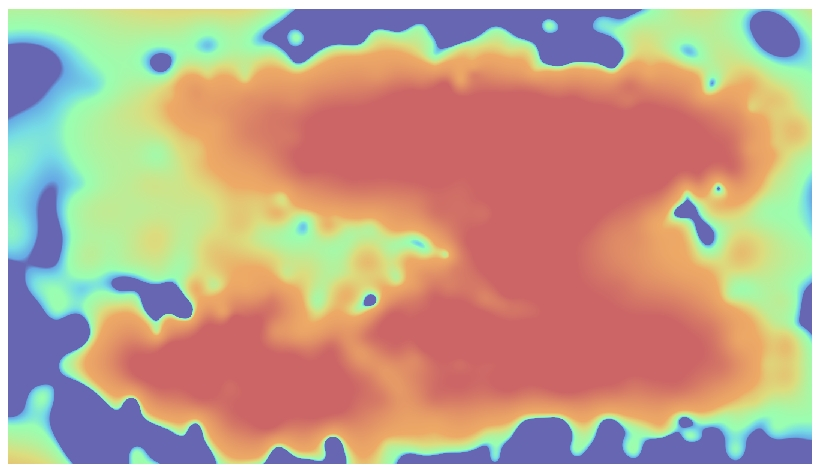
\includegraphics[width=300pt]{./pictures/chagan_spline.jpg}
      \caption[Interpolovaná mapa]{Interpolovaná mapa dávkového příkonu (Chagan Lake) (autor: Tereza Kulovaná, data: \zk{AČR})}
      \label{fig:spline}
\end{figure}

Bodová data pro testování poskytla \zk{AČR}. Jedná se o hodnoty
simulované pro účely cvičení umístěné do oblasti jezera Chagan
(přezdívaného "Atomic lake") v~Kazachstánu. Toto jezero vzniklo v roce
1965 jako důsledek sovětského podzemního jader\-ného testu (ekvivalentní
140 kt TNT) \cite{Nordyke2000}.

Atributová tabulka bodových dat obsahuje informace o měřených
hodnotách dávkového příkonu a plošné aktivity, souřadnicích X a
Y. Interpolovaná mapa dávko\-vého příkonu, resp. plošné aktivity, byla
vytvořena pomocí metody Multilevel B-Spline Interpolation v open
source \zk{GIS} softwaru
SAGA\footnote{\url{http://www.saga-gis.org/saga_tool_doc/2.1.3/grid_spline_4.html}}.
  
\begin{figure}[H] \centering
      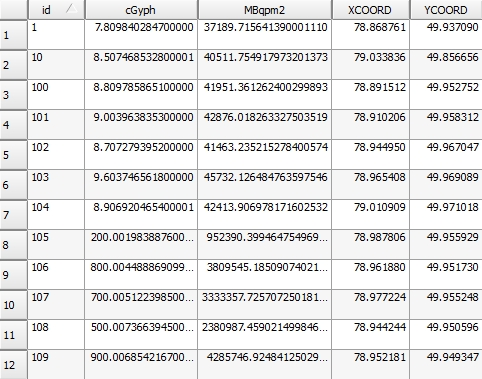
\includegraphics[width=270pt]{./pictures/chagan_attr.jpg}
      \caption[Atributová tabulka bodových dat (Chagan
      Lake)]{Atributová tabulka bodových dat (Chagan Lake) (autor:
        Tereza Kulovaná, data: \zk{AČR})}
      \label{fig:attributes}
\end{figure}

\section{Výstupní data}

\begin{enumerate}
	\item \textbf{Report}

          Povinným výstupem zásuvného modulu je textový report s
          příponou \textit{.txt}, který obsahuje souřadnice lomových
          bodů zjednodušených polygonů v hlásném systému
          \zk{MGRS}. Výstupní report je součástí \zk{MTF} zprávy,
          proto musí splňovat přesně daný formát specifikovaný v
          katalogu APP-11.

\newpage
Jeden řádek reportu obsahuje:

/[VALUE][UNIT]/MGRS:[COORDINATE]/MGRS:[COORDINATE]//

kde
\begin{itemize}
			\item VALUE = hodnota dávkového příkonu/plošné aktivity 
			
			\item UNIT = použitá jednotka ve formátu:
			
			\begin{itemize}
				\item v případě dávkového příkonu: XYH, kde
			 		\begin{itemize}
						\item X = C (\textit{centi}), M (\textit{mili}), U (\textit{mikro})
						\item Y = G (\textit{gray})
						\item H = H (\textit{hodina})
					\end{itemize}
				\item v případě plošné aktivity: BQM2 (\textit{becquerel na čtvereční metr})
			\end{itemize}
			
			\item COORDINATE = souřadnice v systému \zk{MGRS}
\end{itemize}
				
U hodnoty VALUE je oddělovačem desetinných míst desetinná
tečka. Veškerý text musí být velkými písmeny. Report musí začínat
lomítkem, vše mezi dvěma lomítky je nazýváno polem. Pole č. 1 může
obsahovat maximálně 12 znaků. Pole č. 2 může mít až 50 opakování
(maximum 50 souřadnic) a každé pole může za identifikátorem MGRS:
obsahovat maximálně 15 znaků. Poslední souřadnice je zakončena
dvojitým lomítkem (označuje konec řádku). Vše mezi prvním lomítkem a
dvojitým ukončovacím lomítkem se nazývá řádek. Jednotlivé řádky musí
%%% ML: enterem -> zalomeni radky (btw. pouziva se Unixovy nebo Windows zapis?)
být odděleny znakem zalomení řádky.

\begin{figure}[H]
    \centering
      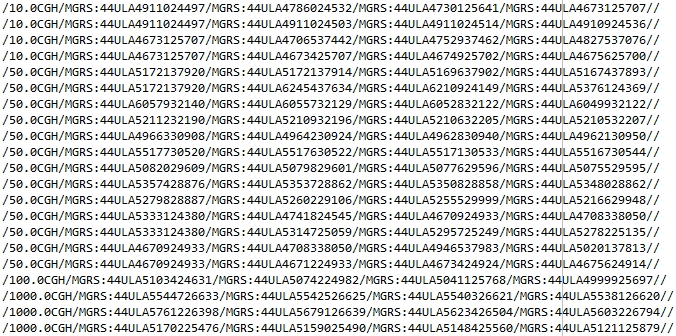
\includegraphics[width=375pt]{./pictures/vystupni_report.jpg}
      \caption[Výstupní report]{Ukázka výstupního reportu (autor: Tereza Kulovaná)}
      \label{fig:report}
\end{figure}

QGIS nemá nativní podporu souřadnic v \zk{MGRS}. Pro převod z \zk{WGS
  84} do \zk{MGRS} byla jako nejvhodnější z dostupných variant zvolena
část kódu již existujícího zásuvného modulu \textit{Lat Lon Tools
  Plugin}\footnote{\url{https://github.com/NationalSecurityAgency/qgis-latlontools-plugin}}. Konkrétně
se jedná o soubor s názvem \texttt{mgrs.py} a v něm obsaženou metodu
\texttt{toMgrs}. Tento zásuvný modul je distribuován pod licencí GNU
\zk{GPL}, stejnou jako vytvářený modul \textit{Radiation
  reconnaissance results}, což umožnilo jeho využití.

	\item \textbf{Soubor polygonů}
	
          Volitelným výstupem zásuvného modulu je datový soubor s
          polygonovými prvky. Data jsou lokalizována v souřadnicovém
          systému \zk{WGS 84} (EPGS:4326) ve formátu Esri Shapefile
          (\textit{.shp}). Datový soubor obsahuje geometrie
          zjednodušených polygonů různě graficky odlišené podle
          jednotlivých úrovní radiace. Atributová tabulka obsahuje:

		\begin{itemize}
			\item{identifikační číslo polygonu}
			\item{úroveň radiace}
		\end{itemize}

%%% ML: symbolizovat podle nejake vhodne skaly?
\begin{figure}[H]
    \centering
      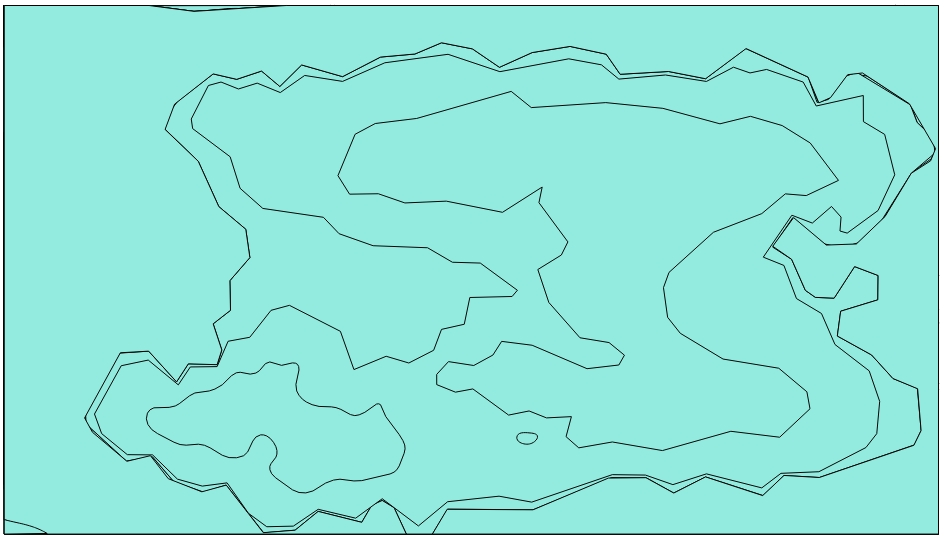
\includegraphics[width=300pt]{./pictures/vystupni_polygony.jpg}
      \caption[Výstupní polygony]{Ukázka výstupního souboru polygonů (autor: Tereza Kulovaná)}
      \label{fig:polygony}
\end{figure}

% obrázek bude upraven (z důvodu správného rozložení stránek)

\end{enumerate}

\section{Tělo zásuvného modulu}

Základní šablona nově vyvíjeného zásuvného modulu byla vytvořena s
pomocí volně dostupného zásuvného modulu \textit{Plugin
  Builder}\footnote{\url{https://plugins.qgis.org/plugins/pluginbuilder/}}. Autorem
tohoto modulu je skupina GeoApt LLC specializující se na rozvoj open
source softwaru. Po zadání povinných vstupních informací
\textit{Plugin Builder} vyprodukuje kostru zásuvného modulu tvořenou
mj. prvotním grafickým uživatelským rozhraním, základními funkcemi,
vazbami a~vychozí ikonkou.

Tuto základní kostru bylo třeba upravit a rozšířit o další soubory,
aby bylo docíleno očekávané funkčnosti. Mezi nejdůležitější prvky
zásuvného modulu patří několik navzájem provázaných souborů:

\begin{itemize}
	\item \textbf{\_\_init\_\_.py} 
	
	Obsahuje základní inicializaci modulu.
		
	\item \textbf{plugin\_upload.py} 

          Umožňuje nahrání modulu do repozitáře QGIS, odkud je
          dostupný komukoli.

	\item \textbf{radiation\_reconnaissance\_results.py} 
	
          Zajišťuje implementaci zásuvného modulu do prostředí QGIS -
          načtení ikonky s~názvem do nástrojové lišty, aktivaci modulu
          a v případě zavření jeho destrukci.

	\item \textbf{radiation\_reconnaissance\_results\_dockwidget.py}
	
          Obstarává propojení se souborem\\
          \textbf{radiation\_reconnaissance\_results\_dockwidget\_base.ui},
          po jehož zavolání se zobrazí grafické uživatelské rozhraní
          vytvořené pomocí Qt Designer. Obsahuje třídu
          \texttt{RadiationReconnaissanceResultsDockWidget} s metodami
          zajišťujícími načtení vstupních dat, předání potřebných
          hodnot dalším výpočetním souborům a v případě volby
          uživatele i přidání výsledné vrstvy polygonů do mapového
          okna. Dále znemožňuje spuštění modulu v situaci, kdy není
          zadána cesta k výstupnímu reportu.

	\item \textbf{pyradiation}

          %%% ML: Zminit, ze jde o knihovnu, ktera neni zavisla na
          %%% QGIS pluginu a muze byt pouzivata mimo nej, to je
          %%% dulezite
          Adresář \textbf{pyradiation} zahrnuje několik vzájemně
          provázaných souborů zajišťujících výpočty a tvorbu
          %%% ML: spise nez o souboru muzete mluvit o "modulu" Jinak
          %%% na tomto miste zminte hlavne dane tridy
          výstupů. V souboru \textbf{isolines.py} jsou ze vstupního
          gridu vytvořeny izolinie v uživatelem zvolených úrovních
          radiace. Datový soubor s~izoliniemi je předán dále do
          \textbf{polygonizer.py}, kde jsou z nich vytvořeny
          zjednodušené polygony pomocí generalizace obsažené v souboru
          \textbf{generalizer.py}. Na závěr jsou v \textbf{report.py}
          souřadnice lomových bodů polygonu převedeny do souřadnic
          systému \zk{MGRS} a v zadaném formátu vypsány do výstupního
          textového reportu.
	
\end{itemize}

\section{Algoritmus}

\begin{figure}[H]
    \centering
      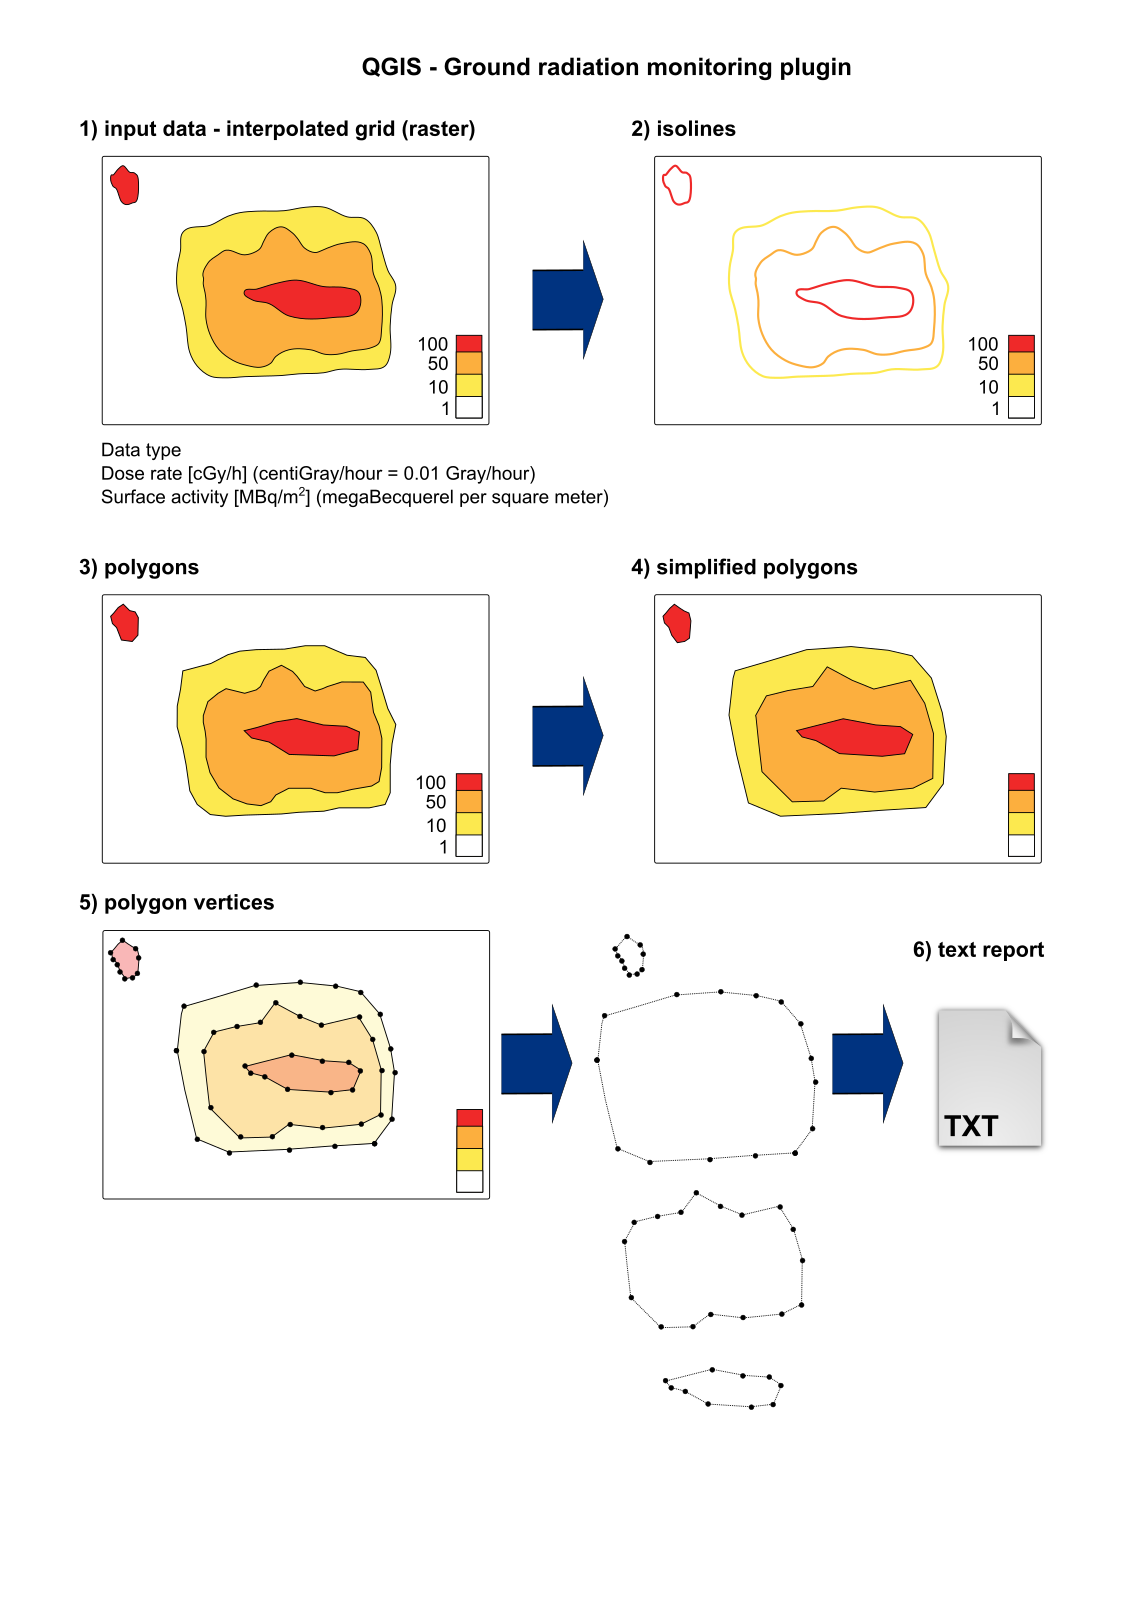
\includegraphics[width=350pt]{./pictures/ACR_radiacni_pruzkum_polygony_v3.png}
      \caption[Schematický postup]{Schematický postup (autor: \zk{SÚRO}, v.v.i.)}
      \label{fig:schema}
\end{figure}

V dalších kapitolách jsou představeny dílčí kroky postupu tvorby
koncových zjednodušených polygonů.

\subsection{Tvorba izolinií}

V první fázi jsou ze vstupního gridu vytvořeny izolinie pomocí metody
\texttt{ContourGenerate} z knihovny \zk{GDAL}. Vstupní grid ovšem
zahrnuje pouze ohraničené pole bez informací z okolí, což v důsledku znamená, že
%%% ML: skutecnost -> okoli ?
část izolinií netvoří uzavřené oblasti, ale začíná a končí na
hranicích gridu a není uzavřena. Z těchto izolinií by nebylo možné
vytvořit polygony, které na vstupu vyžadují uzavřenou oblast. Z tohoto
důvodu je třeba tyto linie najít a uzavřít pomocí ohraničujícího
obdélníku.

V prvním kroku jsou určeny izolinie, které nejsou uzavřené
(pseudokód~\ref{alg:getIntersection}-4), a~pro ně jsou vypočítány
průsečíky s ohraničujícím obdélníkem
(pseudokód~\ref{alg:getIntersection}-5). Tyto průsečíky linií jsou
přidány do pole průsečíků (pseudokód~\ref{alg:getIntersection}-9)
stejně jako rohové body ohraničujícího obdélníku
(pseudokód~\ref{alg:getIntersection}-14). Body v tomto poli jsou
seřazeny proti směru hodinových ručiček
(pseudokód~\ref{alg:getIntersection}-15). Při tvorbě izolinií metodou
\texttt{ContourGenerate} mohou vzniknout i linie, které nejsou
uzavřené a zároveň nekončí na hranicích obdélníka, ty je třeba z
vrstvy izolinií odstranit (pseudokód~\ref{alg:getIntersection}-7).

\begin{algorithm}
\caption{Získání průsečíků s ohraničujícím obdélníkem (Hranice)}
\label{alg:getIntersection}
    \begin{algorithmic}[1] 
    \STATE{vrstvaIzolinie = vrstva izolinií vypočítaných pomocí ContourGenerate}
    \STATE{izolinie = načti první izolinii z vrstvaIzolinie}
    \WHILE{existuje izolinie}
    	\IF{izolinie je neuzavřená}
    		\STATE{průsečík = vypočtiPrůsečíkyIzolinieAHranice}
    		\IF{neexistuje průsečík}		
				\STATE{odstraň izolinii z vrstvaIzolinie}
			\ELSE
				\STATE{přidej průsečík do polePrůsečíky}
			\ENDIF	
		\ENDIF
		\STATE{izolinie = načti další izolinii z vrstvaIzolinie}
	\ENDWHILE
	\STATE{přidej rohové body Hranice do polePrůsečíky}
	\STATE{seřaď polePrůsečíky proti směru hodinových ručiček}
    \end{algorithmic}
\end{algorithm}

V druhém kroku již dochází přímo k uzavírání linií. Základní postup je
přidat první izolinii do nově uzavírané linie
(pseudokód~\ref{alg:closeLines}-4). Pak jsou procházeny průsečíky na
obdélníku, dokud není nalezen další bod se stejnou úrovní radiace
(pseudokód~\ref{alg:closeLines}-9) a linie mezi ním a posledním bodem
je přidána do nově uzavírané linie
(pseudokód~\ref{alg:closeLines}-10). Pokud se jedná o počáteční bod
první izolinie, je linie uzavřená
(pseudokód~\ref{alg:closeLines}-11). Pokud se jedná o bod z jiné
izolinie, je tato izolinie přidána do uzavírané linie
(pseudokód~\ref{alg:closeLines}-24) a znovu se hledá další bod se
stejnou úrovní radiace. Tento postup se opakuje, dokud poslední
přidaný bod neodpovídá počátečnímu bodu první izolinie.


\begin{algorithm}
\caption{Uzavření linií}
\label{alg:closeLines}
    \begin{algorithmic}[1] 
    \STATE{neuzavřenéIzolinie = vrstva neuzavřených izolinií}
    \STATE{izolinie = načti první izolinii z neuzavřenéIzolinie}
    \WHILE{existuje izolinie}
    	\STATE{přidej izolinii do uzavíranáIzolinie}
    	\STATE{počátečníBod = počáteční bod izolinie}
    	\STATE{koncovýBod = koncový bod izolinie}
		\FOR{průsečík z polePrůsečíky}
    		\IF{průsečík po Hranici dál než koncovýBod}	
    			\IF{úroveňPrůsečík = úroveňIzolinie}								
					\STATE{přidej linii mezi koncovýBod a průsečík do uzavíranáIzolinie}
						\IF{průsečík = počátečníBod}
							\STATE{uzavíranáLinie je uzavřena -> \textbf{konec výpočtu}}
						\ELSE
							\STATE{koncovýBod = průsečík}
							\STATE{pokračuj na řádku 22}
						\ENDIF
%					\ELIF{úroveňPrůsečík = 0}
%						\STATE{rohHranice = průsečík}
%						\STATE{přidej linii mezi koncovýBod a rohHranice do uzavíranáIzolinie}
%						\STATE{koncovýBod = rohHranice}
%						\STATE{pokračuj s dalším průsečíkem}
				\ELSE
					\STATE{pokračuj s dalším průsečíkem}
				\ENDIF
			\ENDIF
		\ENDFOR
	\algstore{myalg}
	\end{algorithmic}
\end{algorithm}

\begin{algorithm}
	\begin{algorithmic} [1] \algrestore{myalg}
				\WHILE{uzavíranáLinie není uzavřená}
			\FOR{izolinie z neuzavřenéIzolinie}
				\IF{počátečníBodIzolinie = koncovýBod}
					\STATE{přidej izolinii do uzavíranáIzolinie}
					\STATE{koncovýBod = koncovýBodIzolinie}
					\STATE{pokračuj na řádce 7}
				\ENDIF
			\ENDFOR
		\ENDWHILE
		\STATE{izolinie = načti další izolinii z vrstvaIzolinie}
	\ENDWHILE
    \end{algorithmic}
\end{algorithm}

\newpage
\subsection{Tvorba polygonů}

Z uzavřených izolinií jsou pomocí metody
\texttt{BuildPolygonFromEdges} z knihovny OGR vytvořeny
polygony. Následně jsou zjednodušeny s využitím metody
\texttt{Simplify} ze stejné knihovny. Nakonec jsou souřadnice
zjednodušených polygonů převedeny do systému \zk{MGRS} a vypsány do
textového reportu kompatibilního s formátem dle
APP-11\footnote{\url{https://nhqc3s.hq.nato.int/Apps/Architecture/NISP2/std.aspx?vndb=standards&sbbs=y&refid=nato-app-11-d}}.
%%% TK: Přímo katalog k dispozici nemám.

%%% ML: rozdelit do dvou stranek... (detail, klidne to tak nechate)
\begin{algorithm}
\caption{Tvorba a zjednodušení polygonů}
\label{alg:polygon}
    \begin{algorithmic}[1] 
    \STATE{uzavřenéIzolinie = vrstva uzavřených izolinií}
    \STATE{izolinie = načti první izolinii z uzavřenéIzolinie}
    \WHILE{existuje izolinie}
		\STATE{vytvoř polygon metodou \texttt{BuildPolygonFromEdges}}
		\STATE{tolerance = prvotní volba tolerance}
		\WHILE{True}
			\STATE{zjednoduš polygon metodou \texttt{Simplify} s danou tolerancí}
			\IF{počet bodů v polygonu < 50}
				\STATE{konec}
			\ELSE
				\STATE{tolerance = větší tolerance}
			\ENDIF
		\ENDWHILE	
		\STATE{izolinie = načti další izolinii z vrstvaIzolinie}
	\ENDWHILE
    \end{algorithmic}
\end{algorithm}

%%% ML: po rozdeleni nebude nova stranka treba
\newpage
\subsubsection{Generalizace}
Metoda \texttt{Simplify} z knihovny \zk{GDAL} využívá ke zjednodušení
linie algoritmus Douglas–Peucker (pseudokód~\ref{alg:RDP}). Tento
algoritmus patří k nejčastěji používaným generalizačním algoritmům v
oblasti \zk{GIS}. Na rozdíl od většiny generalizačních algoritmů
neodstraňuje z původní linie body nesplňující geometrickou podmínku,
ale naopak vytváří novou linii tvořenou body, které podmínku splňují.
	
Jedná se o rekurzivní algoritmus, který při zjednodušení řetězce mezi
body \textit{A} a~\textit{B} vezme hranu \textit{AB}. Pokud
nejvzdálenější bod (\textit{C}) původní linie je maximálně ve
vzdálenosti rovnající toleranci \textit{T}, pak je aproximace hrany
dostatečná. V opačném případě rozdělí hranu \textit{AB} v daném bodě
\textit{C}, čímž vzniknou hrany \textit{AC} a \textit{CB}. Ty jsou pak
rekurzivně aproximovány stejným
postupem. \cite{hershberger1992speeding}
	
%	Jedná se o rekurzivní algoritmus, který kolem hrany (spojnice
% dvou bodů z nové linie) hledá body z původní linie mimo koridor o
% zadané toleranci T. Pokud žádný takový nenajde, hrana zůstane
% stejná. Pokud nějaký bod mimo koridor existuje, najde ten, který od
% hrany leží nejdále a vloží ho nové linie. Tím se původní hrana
% rozdělí na dvě. Následně testuje stejnou podmínku na nově
% vytvořených kratších spojnicích.

%%% ML: tady opet text nevychazi dobre...

\begin{figure}[H]
    \centering
      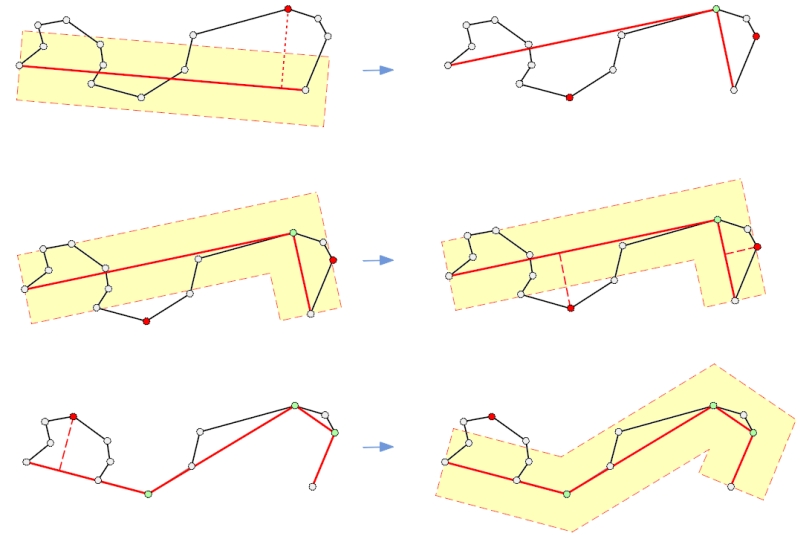
\includegraphics[width=300pt]{./pictures/DPalgoritmus.jpg}
      \caption[Ilustrace DP]{Ilustrace Douglas-Peucker algoritmu (zdroj: Ing. Tomáš Bayer, Ph.D., Přírodovědecká fakulta UK)}
      \label{fig:DPalgo}
\end{figure}
	
\begin{algorithm}
\caption{Douglas–Peuckerův algoritmus}
\label{alg:RDP}
    \begin{algorithmic}[1] 
    \STATE{\textbf{funkce} DouglasPeucker(listBodů[], tolerance)}
    \STATE{dMax = 0}
    \STATE{index = 0}
    \STATE{početBodů = délka(listBodů)}
    \FOR{i = řada od 2 do (početBodů - 1)}
		\STATE{d = vzdálenost(listBodů[i], hrana(listBodů[1], listBodů[početBodů]))}
		\IF{d > dMax}
			\STATE{index = i}
			\STATE{dMax = d}
		\ENDIF	
	\ENDFOR
	\IF{dMax > tolerance}
		\STATE{rekurze1 = DouglasPeucker(listBodů[1...index], tolerance)}
		\STATE{rekurze2 = DouglasPeucker(listBodů[index...početBodů], tolerance)}
		\STATE{výslednýList = {rekurze1[1...délka(rekurze1)-1], rekurze2[1...délka(rekurze2)]}}
	\ELSE
		\STATE{výslednýList = {listBodů[1], listBodů[početBodů]}}
	\ENDIF
	\STATE{\textbf{return} výslednýList[]}
    \end{algorithmic}
\end{algorithm}	

%%% ML: umele pouzit newpage (chtelo by text na poslednich 3-5
%%% strankach vice sladit (az bude finalni)
\newpage		
Tento algoritmus nezachovává vzájemnou polohu linií, je tedy nutné
ještě dalšími úpravami ošetřit, aby se zjednodušené polygony vzájemně
neprotínaly. Tyto úpravy jsou však velmi časově náročné a autorka je
před odevzdáním bakalářské práce nestihla implementovat. Pro správnou
funkčnost zásuvného modulu jsou však nutné a bude na nich pokračovat
po odevzdání.

\chapter{Závěr}
\label{5-zaver}

%Na čem se dá ještě dál pracovat:
%generalizace
%interpolace
%zpracování bodových dat (ne rastru)

Tato bakalářská práce si kladla za cíl tvorbu zásuvného modulu
automatizujícího zpracování dat získaných v rámci terénního radiačního
průzkumu a jeho implementaci do prostředí QGIS. Požadavek na tvorbu
tohoto softwarového nástroje vznesla Armáda ČR, jejíž operátoři dosud
zpracovávali naměřená data ručně. Práce byla doplněna o teoretickou
část s úmyslem seznámit čtenáře se základními informacemi o radiačním
průzkumu.

V současnosti zásuvný modul umožňuje ze vstupní interpolované mapy
dávkového příkonu či plošné aktivity vytvořit izolinie v uživatelem
navolených úrovních. Ty jsou následně převedeny na polygony. Poté je
provedena generalizace jednotlivých polygonů na max. počet bodů = 50
(hodnota vychází z požadavků na výstup). Ty jsou převedeny do
souřadnic systému \zk{MGRS} a vypsány do textového reportu
kompatibilního s formátem dle katalogu APP-11. Uživatel si může sám
zvolit, zda chce vytvořit soubor s grafickým znázorněním polygonů ve
formátu ESRI SHAPEFILE. Nástroj i návod k jeho použití jsou v
anglickém jazyce, protože v případě, že se osvědčí, existuje možnost
jeho využití i v zahraničních institucích.

Při tvorbě zásuvného modulu nastalo několik případů, kdy bylo nutno
změnit zvolený postup či kontaktovat zadavatele pro upřesnění
informací. Tím se zpracování prodloužilo, kvůli čemuž u zjednodušených
polygonů prozatím není ošetřeno, aby se vzájemně neprotínaly. Tyto
úpravy jsou pro správnou funkčnost zásuvného modulu dle zadání nutné,
ale zároveň je jejich implementace časově náročná. Autorka na nich
bude pracovat po odevzdání práce.

Jako další vylepšení modulu v budoucnosti se nabízí rozšíření
vstupních formátů o naměřená bodová data a jejich následnou
interpolaci (pravděpodobně s využitím SAGA-GIS nebo GRASS GIS
\zk{API}). Studiu těchto postupů se autorka věnovala v počátcích
práce, kdy se ještě uvažovalo o zapracování této funkce do zásuvného
modulu v rámci bakalářské práce. S ohledem na časovou náročnost od
implementace bylo upuštěno, ale je možnost se k ní vrátit, až bude
modul plně funkční.

Zásuvný modul využívá knihoven QGIS a musí být distribuován pod
stejnou licencí, tedy GNU \zk{GPL}. Modul je volně dostupný v
repozitáři CTU GeoForAll
Lab\footnote{https://github.com/ctu-geoforall-lab-projects/bp-kulovana-2017},
zde jsou uveřejněna i testovací data. Po jeho dokončení bude začleněn
do oficiálního QGIS repozitáře.


% Vysázení seznamu zkratek

\begin{seznamzkratek}{ABCDE}

	\novazkratka{SÚRO}
	      {SÚRO}
	      {Státní ústav radiační ochrany, v.v.i.}
	      
	 \novazkratka{AČR}	
	     {AČR}
	     {Armáda České republiky (Army of the Czech republic)}	  
	     
	\novazkratka{SÚJB}
	      {SÚJB}
	      {Státní ústav pro jadernou bezpečnost}
	      
	\novazkratka{ČHMÚ}
	      {ČHMÚ}
	      {Český hydrometeorologický úřad}	         
	      
	\novazkratka{PSF}
		  {PSF}
	      {Python Software Foundation}

	\novazkratka{GIS}
	      {GIS}
	      {Geografický informační systém (Geographic information system)}
	         
	  \novazkratka{GUI}	
	      {GUI}
	      {Grafické uživatelské rozhraní (Graphical user interface)}
	           
	  \novazkratka{WGS 84}	
	      {WGS 84}
	      {Světový geodetický systém 1984 (World Geodetic System 1984)}

	  \novazkratka{GPL}	
	      {GPL}
	      {Všeobecná veřejná licence (General Public License)}
	      
	  \novazkratka{LGPL}	
	      {LGPL}
	      {Lesser General Public License}	      
	      
	  \novazkratka{GDAL}	
	      {GDAL}
	      {Geospatial Data Abstraction Library}
	      
	  \novazkratka{API}	
	      {API}
	      {Rozhraní pro programování aplikací (Application program interface)}	      
	    
	  \novazkratka{MGRS}	
	      {MGRS}
	      {Military grid reference system}
	      
	  \novazkratka{NATO}	
	      {NATO}
	      {Severoatlantická aliance (North Atlantic Treaty Organization)}
	      
	  \novazkratka{UTM}	
	      {UTM}
	      {Univerzální transverzální Mercatorův systém souřadnic (Universal Transverse Mercator)}	
	      
	  \novazkratka{UPS}	
	      {UPS}
	      {Universal polar stereographic}	
	      
	   \novazkratka{ALARA}	
	      {ALARA}
	      {As Low As Reasonably Achievable}     
	      
	   \novazkratka{OSGeo}	
	      {OSGeo}
	      {Open Source Geospatial Foundation} 
	      
	   \novazkratka{RMS}	
	      {RMS}
	      {Radiační monitorovací síť}	  
	     	  
	 	\novazkratka{PFDE}	
	      {PFDE}
	      {Příkon fotonového dávkového ekvivalentu}
	     	  
	 	\novazkratka{PPDE}	
	      {PPDE}
	      {Příkon prostorového dávkového ekvivalentu}
	     	  
	 	\novazkratka{ZHN}	
	      {ZHN}
	      {Zbraně hromadného ničení}
	     	     	  
	 	\novazkratka{JE}	
	      {JE}
	      {Jaderná elektrárna}
	     	  
	 	\novazkratka{MonRaS}	
	      {MonRaS}
	      {Program pro monitorování radiační situace}
	     	  
	 	\novazkratka{SVZ}	
	      {SVZ}
	      {Síť včasného zajištění}
	     	  
	 	\novazkratka{SVZ ARMS}	
	      {SVZ ARMS}
	      {Síť včasného zjištění Armádní radiační monitorovací sítě}
	      
	 	\novazkratka{TDS}	
	      {TDS}
	      {Teledozimetrický systém}	   
	      
	 	\novazkratka{MTF}	
	      {MTF}
	      {the Message Text Format}	         
	      	            	      

\end{seznamzkratek}

% Literatura
\nocite{*}
\def\refname{Literatura}
\bibliographystyle{mystyle}
\bibliography{literatura}


% Začátek příloh
\def\figurename{Figure}%
\prilohy

% Vysázení seznamu příloh
%\seznampriloh

% Vložení souboru s přílohami
%%%%%%%%%%%%%%%%%%%%%%%%%%%%%%%%%%%%%%%%%%%%%%%%%%%%%%%%%%%%%%%%%%%%%%%%%%%%%%%%%%%
%%                 PŘÍLOHA - UŽIVATELSKÁ PŘÍRUČKA                                %%
%%%%%%%%%%%%%%%%%%%%%%%%%%%%%%%%%%%%%%%%%%%%%%%%%%%%%%%%%%%%%%%%%%%%%%%%%%%%%%%%%%%
\chapter{User guide}
\label{user-guide}

This user guide is ...

\section{Loading of plugin}
\label{plugin-load}




% Konec dokumentu
\end{document}
